\begin{frame}{Contents}
   \begin{itemize}
       \item[\textcolor{red}{$\checkmark$}] Chisel の導入
       \item[\textcolor{red}{$\checkmark$}] Pros. \& Cons.
       \item[\textcolor{red}{$\checkmark$}] ChiselImProc の説明
       \item[\textcolor{red}{$\rhd$}] Vivado HLS との比較
   \end{itemize} 
\end{frame}



\begin{frame}{Lenna の画像によるテストベンチ}
    \begin{columns}[t, onlytextwidth]
        \begin{column}{0.5\textwidth}
            Vivado HLS
            \begin{figure}
                \centering
                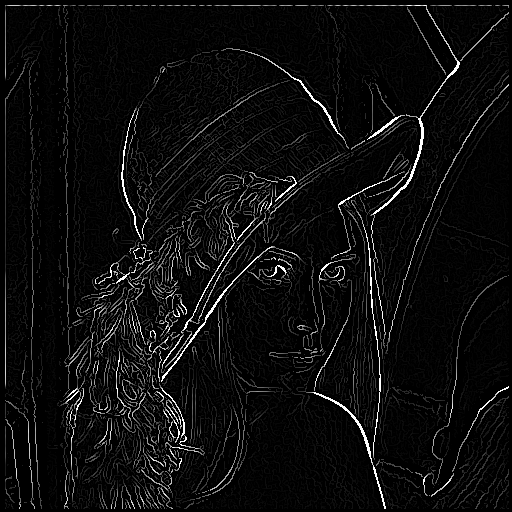
\includegraphics[width=0.9\textwidth]{./figures/out_hls.png}
            \end{figure}
        \end{column}
        \begin{column}{0.5\textwidth}
            Chisel
            \begin{figure}
                \centering
%                \begin{overpic}[grid,width=0.9\textwidth]{./figures/out_original.png}
%                \end{overpic}
                \only<1>{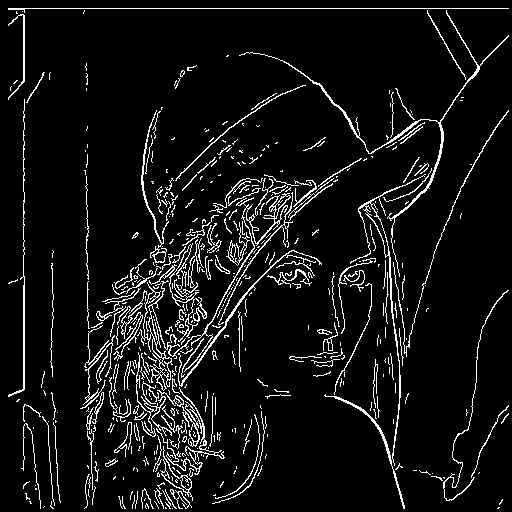
\includegraphics[width=0.9\textwidth]{./figures/out_original.png}}
                \only<2>{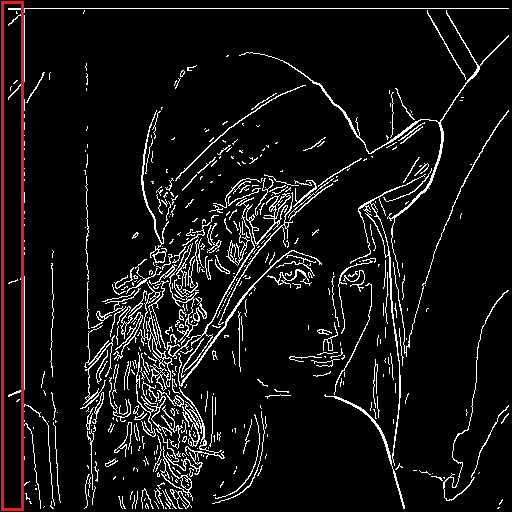
\includegraphics[width=0.9\textwidth]{./figures/out_original_edit.png}}
            \end{figure}
        \end{column}
    \end{columns}
    \begin{itemize}
        \item HLS のほうだとなぜか2値になっていない
        \item last信号の処理が甘いため20ピクセルほどずれる
    \end{itemize}
    
    
\end{frame}


\begin{frame}{Implementation後のUtilization}
\begin{columns}[t,onlytextwidth]
    \begin{column}{0.5\textwidth}
        Vivado HLS
        \begin{figure}
            \centering
            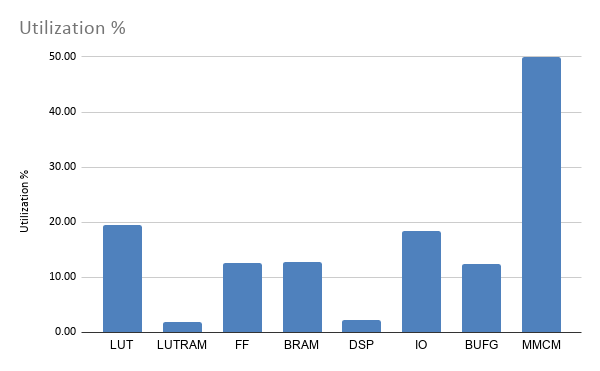
\includegraphics[width=\textwidth]{./figures/Utilization_hls.png}
        \end{figure}
    \end{column}
    \begin{column}{0.5\textwidth}
        Chisel
        \begin{figure}
            \centering
            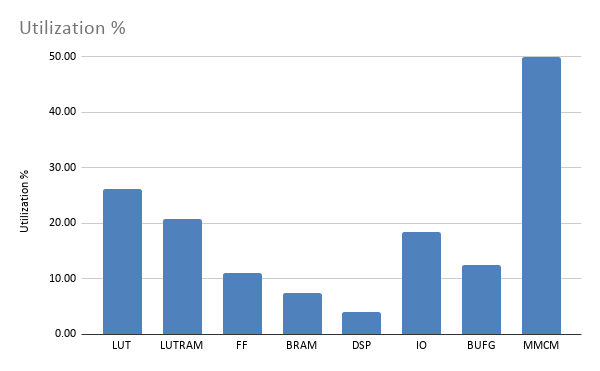
\includegraphics[width=\textwidth]{./figures/Utilization_chisel.png}
        \end{figure}
    \end{column}
\end{columns}

ChiselのBRAMはSystem ila ($+15 \sim 20$\%) が含まれる。
    
\end{frame}

